% Compile with latex, then dvisvgm --no-fonts --exact --bbox=min.
\documentclass[tikz,border=5pt]{standalone}
\begin{document}
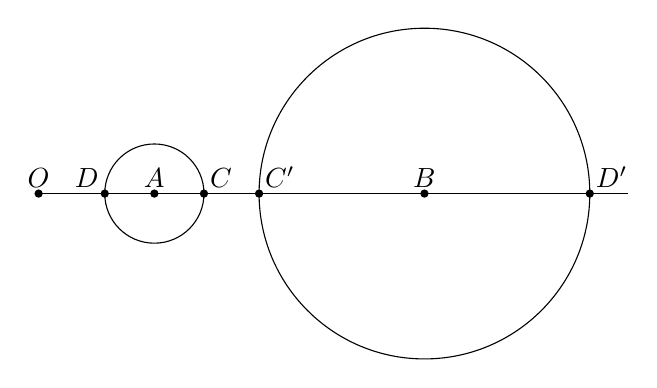
\begin{tikzpicture}[x=0.7cm,y=0.7cm,every node/.style={inner sep=0pt}]
  % OD=1.2, OC=3, OC'=4, OD'=10: both products equal R^2=12.
  \draw (2.1,0) circle (0.9);
  \draw (7,0) circle (3);
  \draw (0,0) -- (10.7,0);
  \foreach \x in {0,1.2,2.1,3,4,7,10} {
    \fill (\x,0) circle (1.5pt);
  }
  \node[above=2pt] at (0,0) {$O$};
  \node[above=2pt] at (2.1,0) {$A$};
  \node[above=2pt] at (7,0) {$B$};
  % Keep boundary labels close to their points and clear of the outlines.
  \node[above left=2pt] at (1.2,0) {$D$};
  \node[above right=2pt] at (3,0) {$C$};
  \node[above right=2pt] at (4,0) {$C'$};
  \node[above right=2pt] at (10,0) {$D'$};
\end{tikzpicture}
\end{document}
